\documentclass{beamer}
% \DeclareMathOperator{\Sample}{Sample}
\let\vaccent=\v % rename builtin command \v{} to \vaccent{}
\renewcommand{\v}[1]{\ensuremath{\mathbf{#1}}} % for vectors
\newcommand{\gv}[1]{\ensuremath{\mbox{\boldmath$ #1 $}}} 
% for vectors of Greek letters
\newcommand{\uv}[1]{\ensuremath{\mathbf{\hat{#1}}}} % for unit vector

\let\underdot=\d % rename builtin command \d{} to \underdot{}
\renewcommand{\d}[2]{\frac{d #1}{d #2}} % for derivatives
\newcommand{\dd}[2]{\frac{d^2 #1}{d #2^2}} % for double derivatives
\newcommand{\pd}[2]{\frac{\partial #1}{\partial #2}} 
% for partial derivatives
\newcommand{\pdd}[2]{\frac{\partial^2 #1}{\partial #2^2}} 
% for double partial derivatives
\newcommand{\pddm}[3]{\frac{\partial^2 #1}{\partial #2 \: \partial #3}}
% for mixed double partial derivatives
\newcommand{\pdc}[3]{\left( \frac{\partial #1}{\partial #2}
 \right)_{#3}} % for thermodynamic partial derivatives
\newcommand{\ket}[1]{\left| #1 \right>} % for Dirac bras
\newcommand{\bra}[1]{\left< #1 \right|} % for Dirac kets
\newcommand{\braket}[2]{\left< #1 \vphantom{#2} \right|
 \left. #2 \vphantom{#1} \right>} % for Dirac brackets
\newcommand{\matrixel}[3]{\left< #1 \vphantom{#2#3} \right|
 #2 \left| #3 \vphantom{#1#2} \right>} % for Dirac matrix elements
\newcommand{\xval}[1]{\left\langle #1 \right\rangle} % for expectation values

\newcommand{\abv}[1]{\lvert #1 \rvert}

\mode<presentation> {
% The Beamer class comes with a number of default slide themes
% which change the colors and layouts of slides. Below this is a list
% of all the themes, uncomment each in turn to see what they look like.

%\usetheme{default}
%\usetheme{AnnArbor}
%\usetheme{Antibes}
%\usetheme{Bergen}
%\usetheme{Berkeley}
%\usetheme{Berlin}
\usetheme{Boadilla}
%\usetheme{CambridgeUS}
%\usetheme{Copenhagen}
%\usetheme{Darmstadt}
%\usetheme{Dresden}
%\usetheme{Frankfurt}
%\usetheme{Goettingen}
%\usetheme{Hannover}
%\usetheme{Ilmenau}
%\usetheme{JuanLesPins}
%\usetheme{Luebeck}
%\usetheme{Madrid}
%\usetheme{Malmoe}
%\usetheme{Marburg}
%\usetheme{Montpellier}
%\usetheme{PaloAlto}
%\usetheme{Pittsburgh}
%\usetheme{Rochester}
%\usetheme{Singapore}
%\usetheme{Szeged}
%\usetheme{Warsaw}

% As well as themes, the Beamer class has a number of color themes
% for any slide theme. Uncomment each of these in turn to see how it
% changes the colors of your current slide theme.

%\usecolortheme{albatross}
%\usecolortheme{beaver}
%\usecolortheme{beetle}
%\usecolortheme{crane}
%\usecolortheme{dolphin}
%\usecolortheme{dove}
%\usecolortheme{fly}
%\usecolortheme{lily}
%\usecolortheme{orchid}
%\usecolortheme{rose}
%\usecolortheme{seagull}
%\usecolortheme{seahorse}
%\usecolortheme{whale}
%\usecolortheme{wolverine}

%\setbeamertemplate{footline} % To remove the footer line in all slides uncomment this line
%\setbeamertemplate{footline}[page number] % To replace the footer line in all slides with a simple slide count uncomment this line

%\setbeamertemplate{navigation symbols}{} % To remove the navigation symbols from the bottom of all slides uncomment this line
}

\usepackage{graphicx}
\usepackage{subcaption}
\usepackage{amsmath}
\usepackage{amssymb}

%-------------------------------------------------------------------------------
% TITLE SLIDES
%-------------------------------------------------------------------------------
\title[Criticality]{Criticality \& information transfer in neural networks}
\date{December 6, 2013}
\author[P. Rozdeba \and F. Sheldon]{Paul Rozdeba\\ \and Forrest Sheldon}
\institute[UCSD]{University of California, San Diego}
\begin{document}
\begin{frame}
\titlepage
\end{frame}

%-------------------------------------------------------------------------------
% PRESENTATION SLIDES
%-------------------------------------------------------------------------------
\begin{frame}
\frametitle{What is Criticality?}
\begin{itemize}

\item<1> Anything with a power law.
\item<2> But really...
\item<3> Near a critical phase transition, as we vary a parameter of the system
the correlation lengths diverge in space and the dynamics slow. The spartial correlations take the form of power law distributions.
\item<3>The canonical example
\begin{figure}
	\centering
	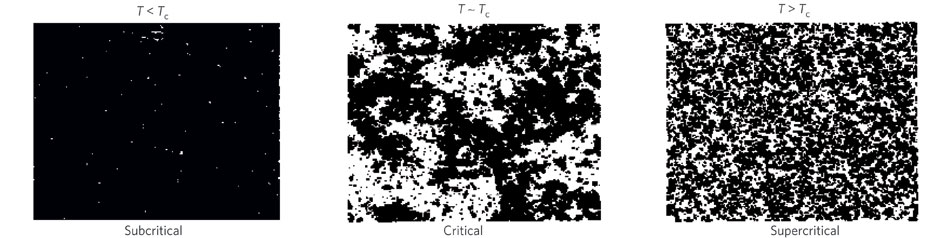
\includegraphics[width=.9\textwidth]{Ising_critical}
\end{figure}
\end{itemize}
\end{frame}

%-------------------------------------------------------------------------------

\begin{frame}
\frametitle{The case for Criticality in Neuroscience}
From Chialvo, Emergent Complex Dynamics, Nature Physics 6 2010:
\begin{itemize}
\item Brain has necessary hardware to show criticalty
\item Healthy brains lack a preferred time scale
\item fMRI degree distributions are power-law
\item Neuronal avalances have power law size distributions
\item All known models that display complex emergent behavior display criticality
\end{itemize}
These arguments all make the case for a resemblance but lack any reason why an
organism would want a critical nervous system.
\end{frame}

%-------------------------------------------------------------------------------

\begin{frame}
\frametitle{Hypothesis}
The dynamics of systems near a critical phase transition enhance information propagation through the system and naturally enact certain encoding strategies.
\newline
\newline
To this end we (are) examining simple systems that display a critical transition:
\newline
\newline
Does the Ising model naturally perform compressive sensing but only near the phase transition?
\newline
\newline
Is dynamical synchronization to a measured signal optimized near criticality?

\end{frame}

%-------------------------------------------------------------------------------

\begin{frame}
\frametitle{Neural network: dynamical model}
A model of $N$ interconnected ``neurons'' that obey the dynamics:
\begin{align*}
	\d{V_i}{t} = -V_i + \sum_j J_{ij} S_j
\end{align*}
where $S_i$ is the ``activity'' of a neuron, defined as
$$ S_i \equiv tanh(g\tilde{J}V_i). $$
Actually it might as well be any sigmoidal function of $V_i$.  The sigmoidal behavior limits the coupling to avoid runaway unstable solutions (also biophysically motivated, like a saturation of the interneuronal coupling).
\end{frame}

%-------------------------------------------------------------------------------

\begin{frame}
\frametitle{Random neural network: dynamical model}
The randomness lies in $J_{ij}$.  Each entry is a Gaussian-distributed random variable with the statistics
\begin{align*}
	\left\langle J_{ij} \right\rangle &= 0 \\
	\left\langle J_{ij} J_{kl} \right\rangle &= \frac{\tilde{J}^2}{N} \delta_{ik}\delta_{jl}.
\end{align*}
In general, the dynamics of this kind of system are non-relaxational (i.e. the system does not converge to a global minimum of an energy function) since the couplings are asymmetric.
\newline
\newline
In the large-$N$ limit, the dynamics can be reduced to the form
$$ \d{V_i}{t} = -V_i + \eta_i $$
and there exist a broad range of chaotic solutions.

\end{frame}

%-------------------------------------------------------------------------------

\begin{frame}
\frametitle{Random neural network: dynamical model}
With these definitions, the quantity $g\tilde{J}$ acts like a control parameter for the dynamics of the quantity
$$ \Delta(t) \equiv \left\langle V_i(t_0+t) V_i(t_0) \right\rangle $$
Roughly, when $g\tilde{J}$ crosses above 1, the dynamics undergo a qualitative change in behavior that looks much like the phase transition in the Ising model; $\Delta$ acts as a qualifier for the behavior.
\end{frame}

%-------------------------------------------------------------------------------

\begin{frame}
\frametitle{$g\tilde{J} = 1.1$}
\begin{figure}
	\centering
	\begin{subfigure}[b]{0.49\textwidth}
		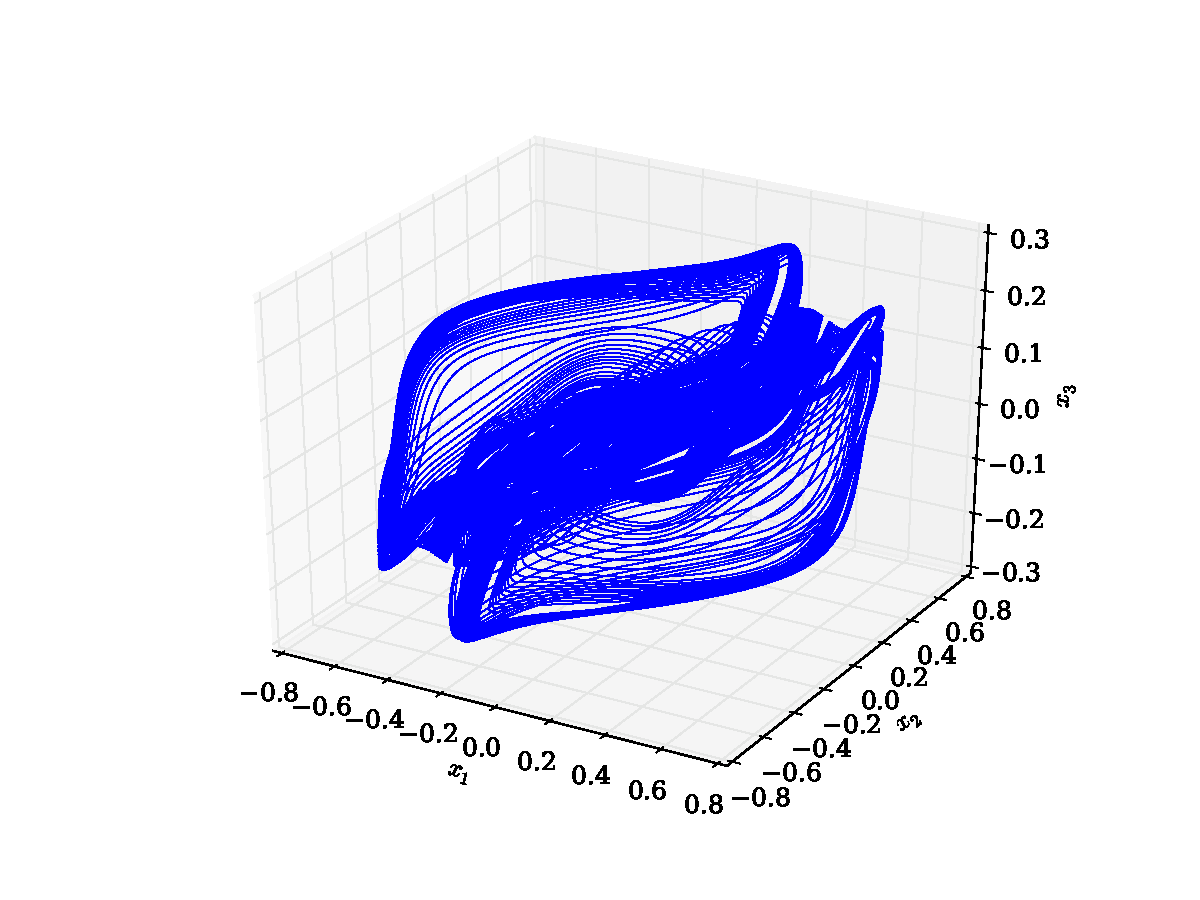
\includegraphics[width=\textwidth]{paulfigs/J_1_1_3d}
	\end{subfigure}
	\begin{subfigure}[b]{0.49\textwidth}
		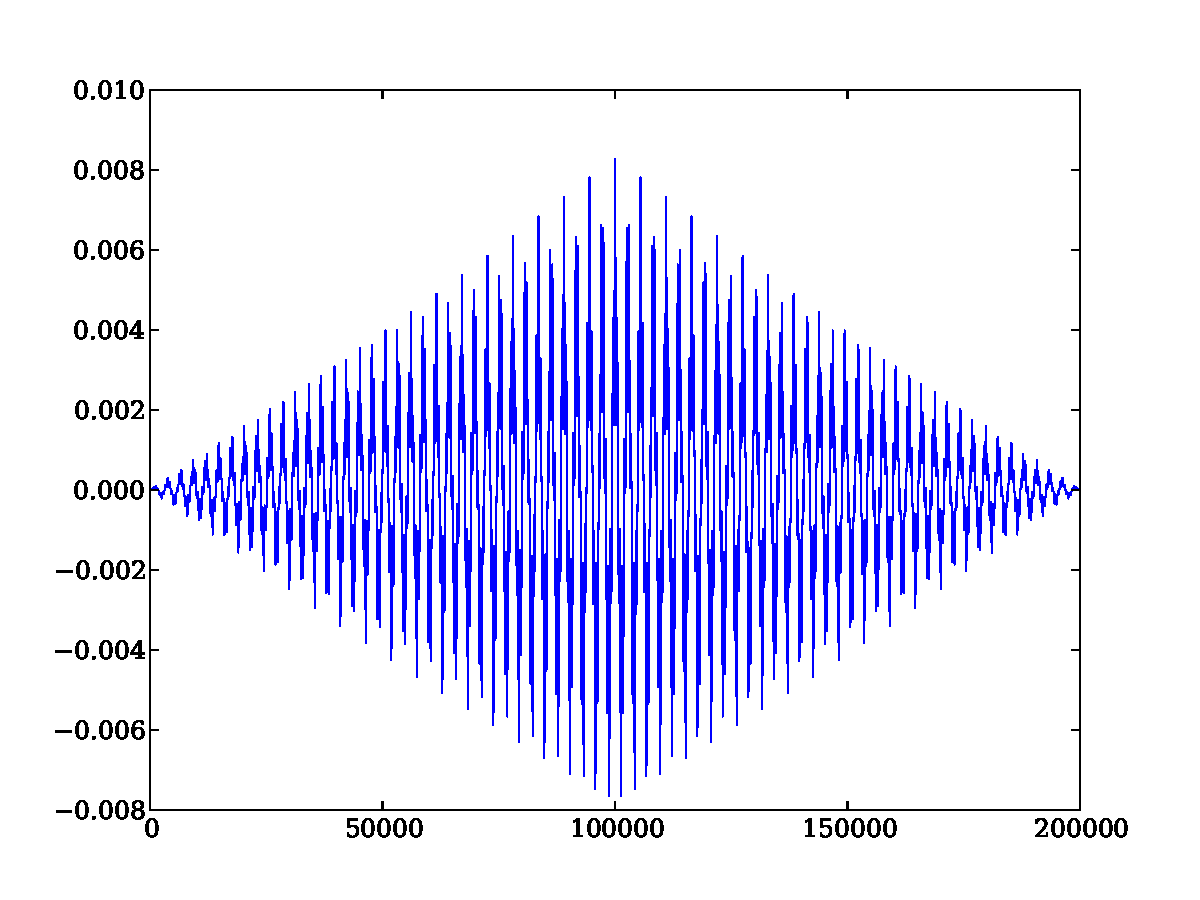
\includegraphics[width=\textwidth]{paulfigs/tcorr_J_1_1}
	\end{subfigure}
\end{figure}
\end{frame}

%-------------------------------------------------------------------------------

\begin{frame}
\frametitle{$g\tilde{J} = 1.2$}
\begin{figure}
	\centering
	\begin{subfigure}[b]{0.49\textwidth}
		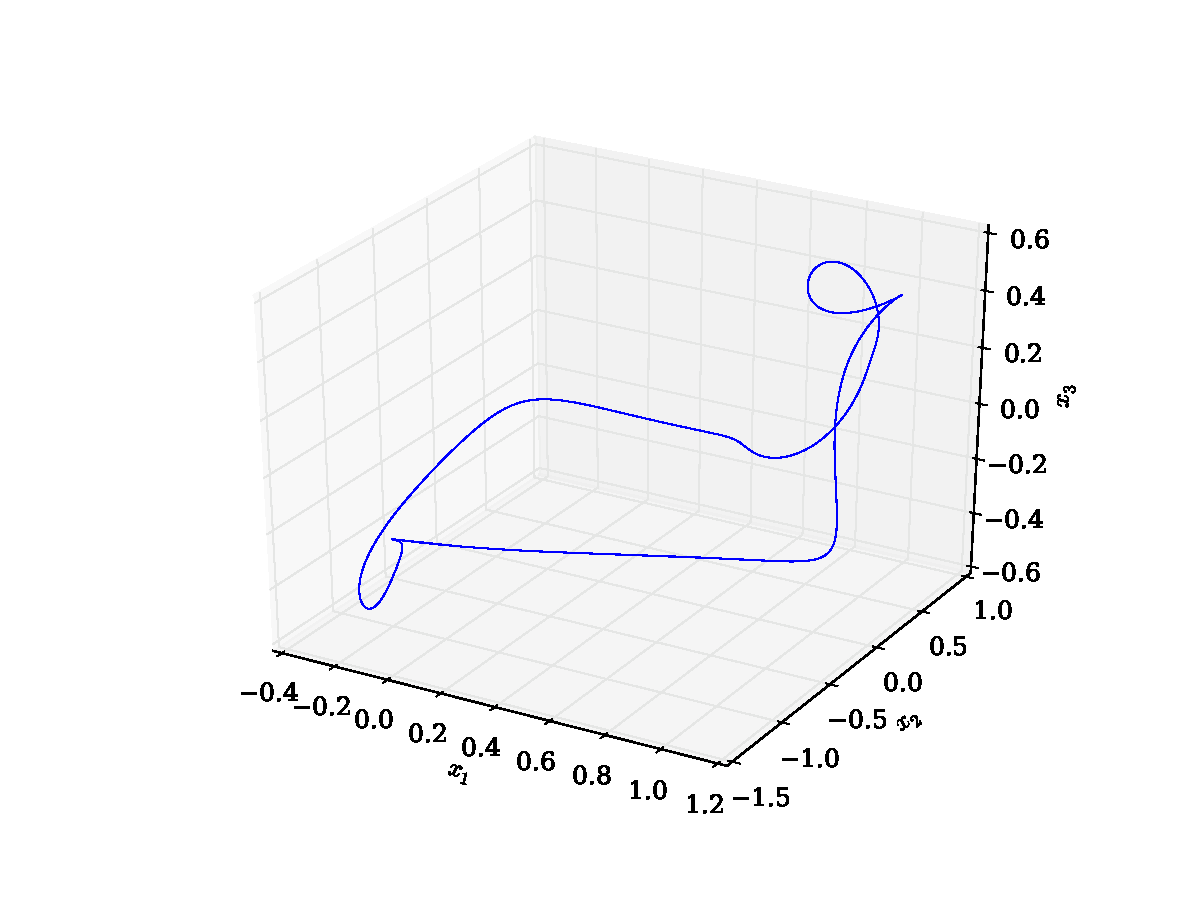
\includegraphics[width=\textwidth]{paulfigs/J_1_2_3d}
	\end{subfigure}
	\begin{subfigure}[b]{0.49\textwidth}
		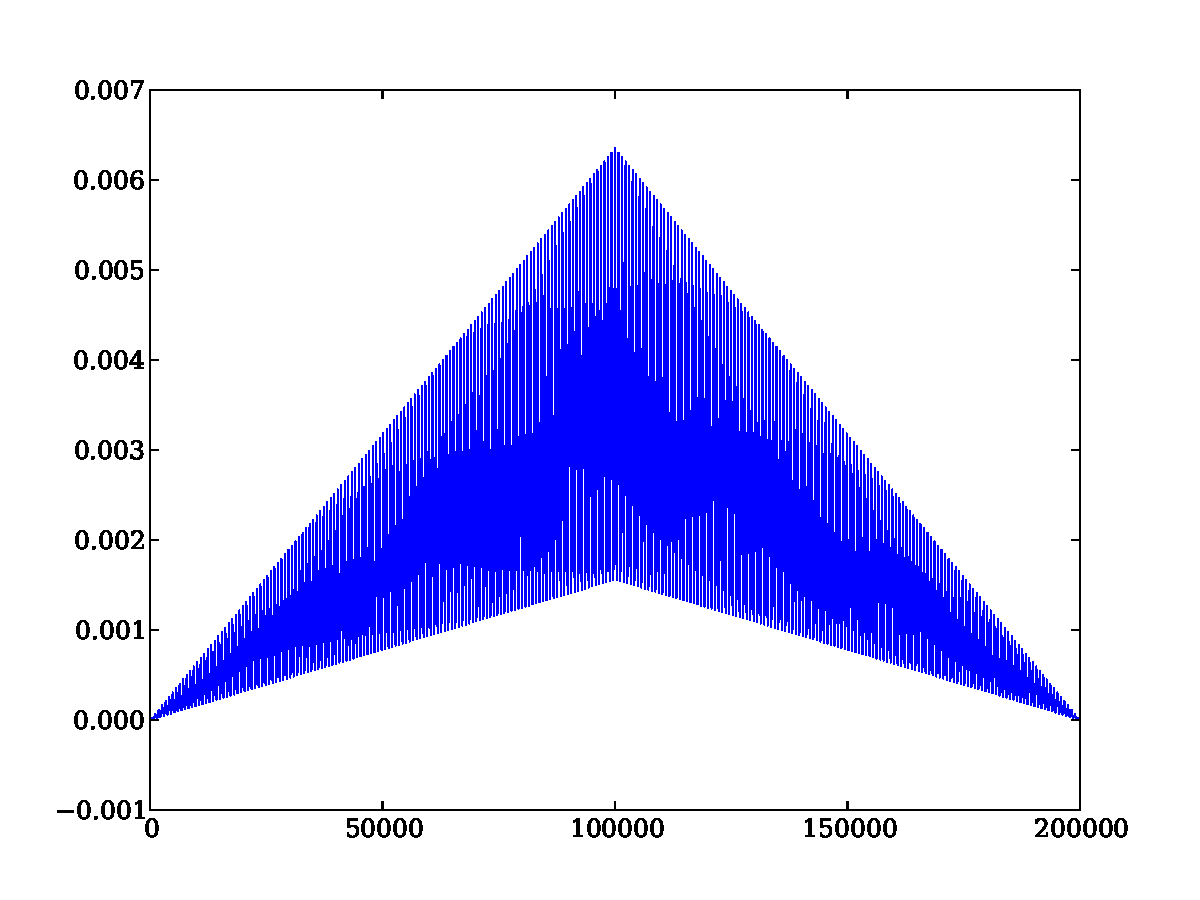
\includegraphics[width=\textwidth]{paulfigs/tcorr_J_1_2}
	\end{subfigure}
\end{figure}
\end{frame}

%-------------------------------------------------------------------------------

\begin{frame}
\frametitle{$g\tilde{J} = 1.26$}
\begin{figure}
	\centering
	\begin{subfigure}[b]{0.49\textwidth}
		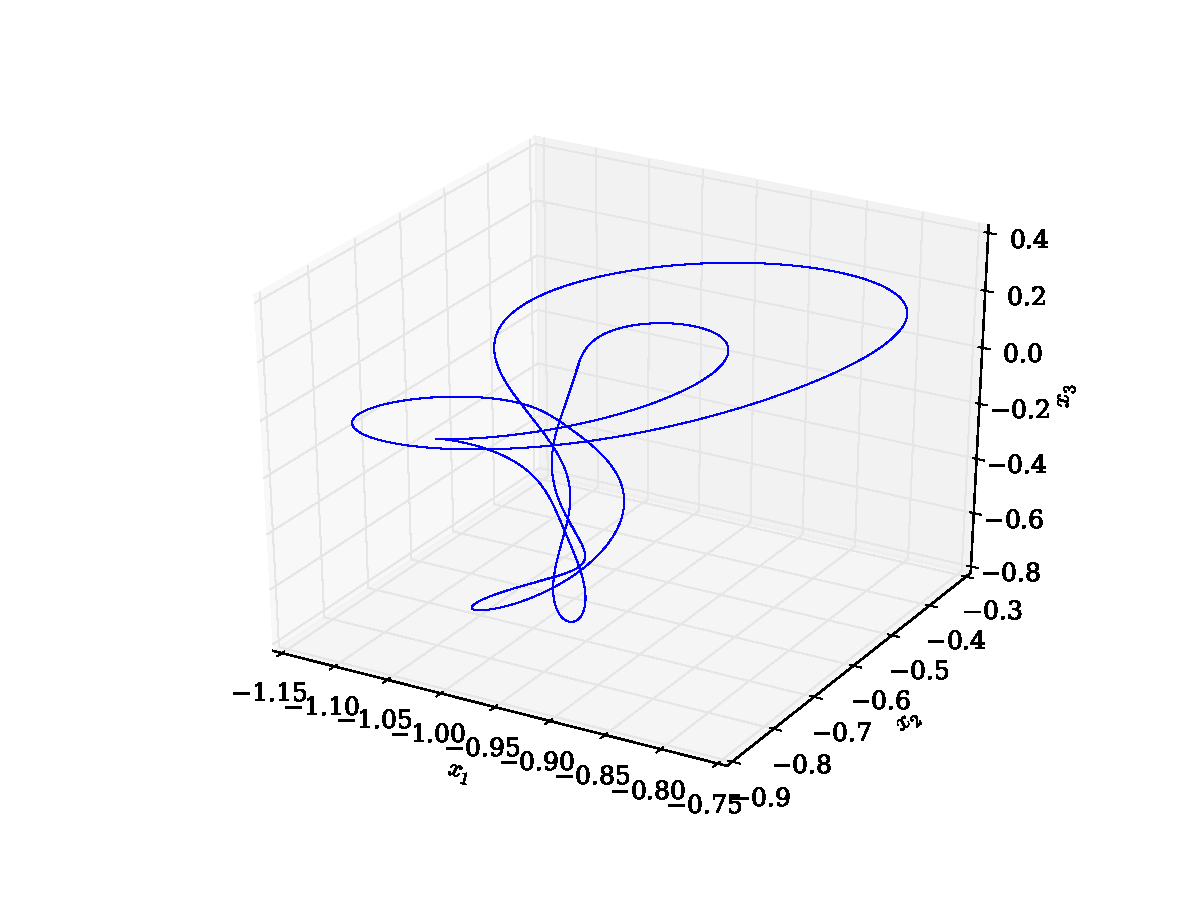
\includegraphics[width=\textwidth]{paulfigs/J_1_26_3d}
	\end{subfigure}
	\begin{subfigure}[b]{0.49\textwidth}
		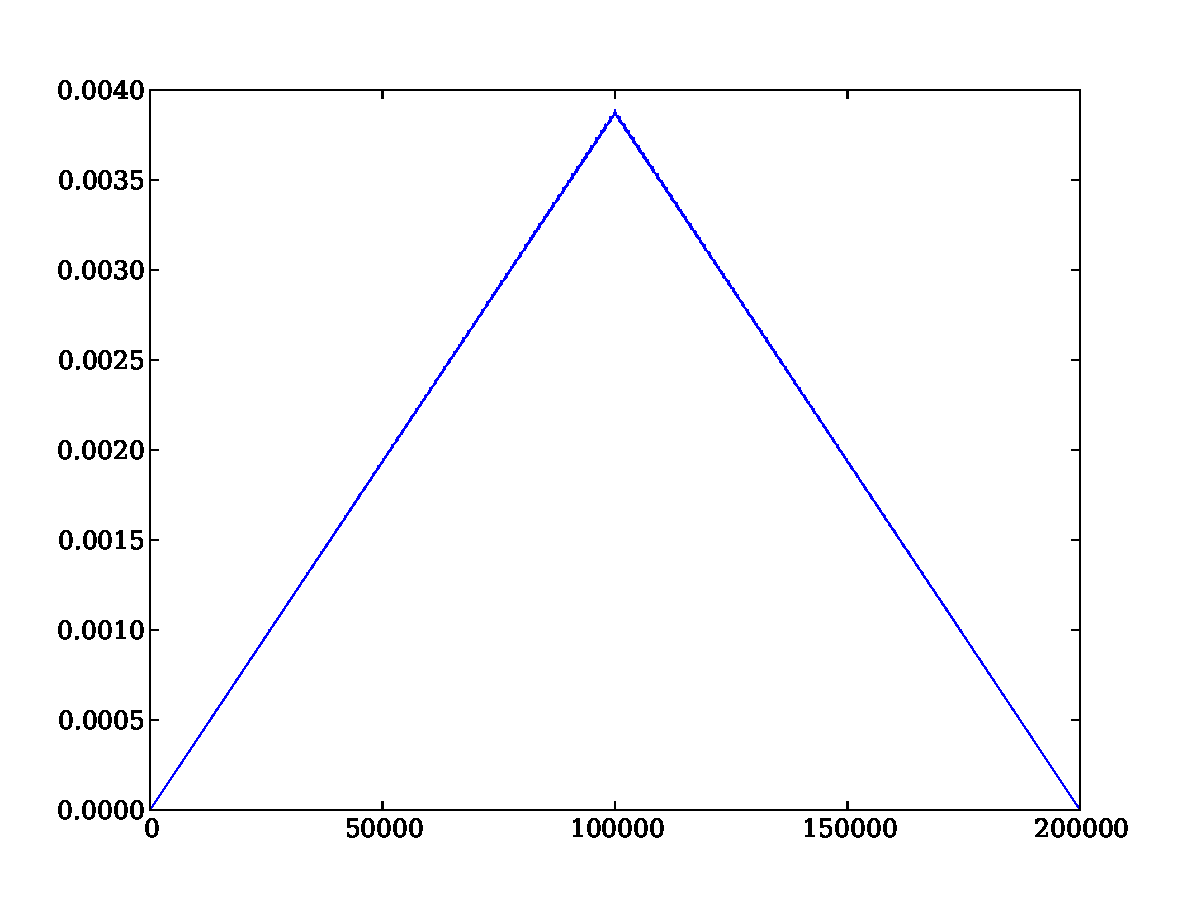
\includegraphics[width=\textwidth]{paulfigs/tcorr_J_1_26}
	\end{subfigure}
\end{figure}
\end{frame}

%-------------------------------------------------------------------------------

\begin{frame}
\frametitle{$g\tilde{J} = 1.266$}
\begin{figure}
	\centering
	\begin{subfigure}[b]{0.49\textwidth}
		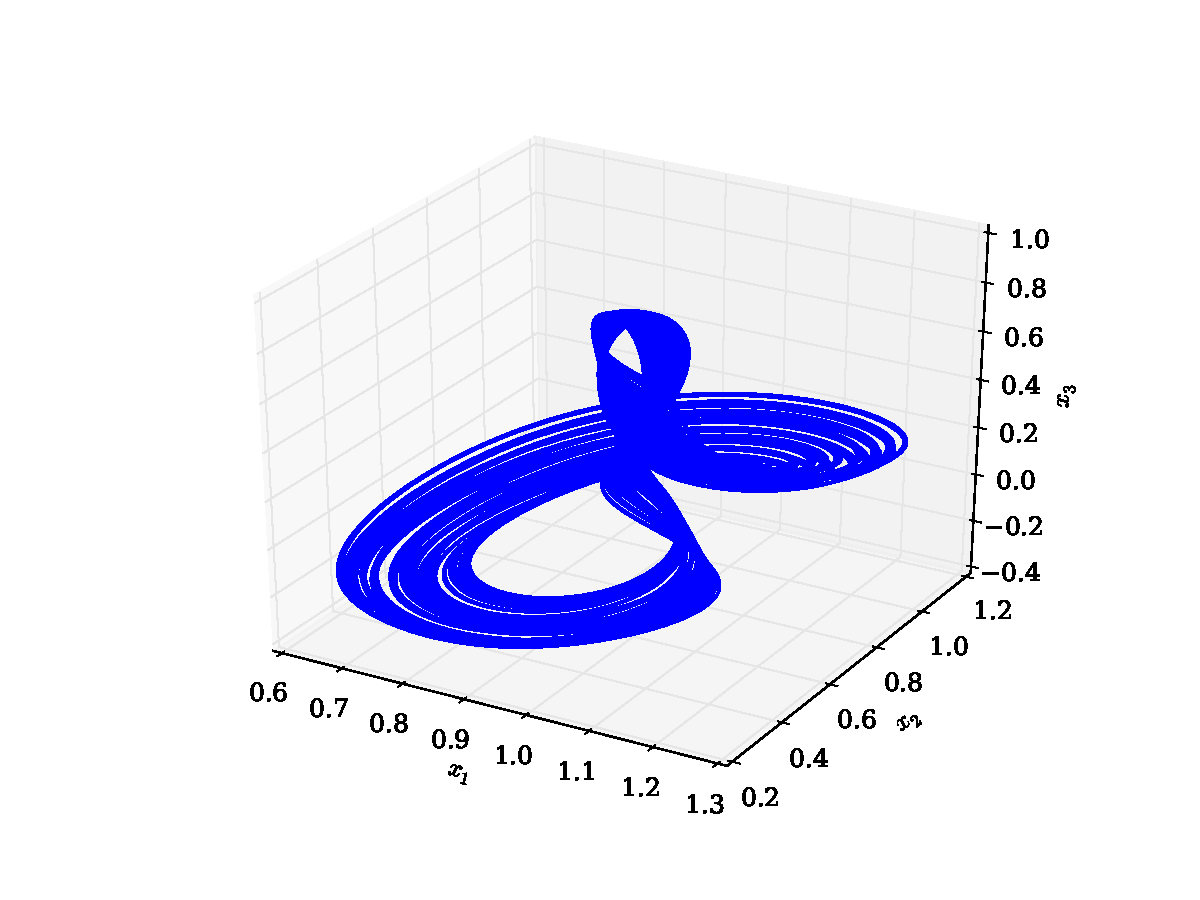
\includegraphics[width=\textwidth]{paulfigs/J_1_266_3d}
	\end{subfigure}
	\begin{subfigure}[b]{0.49\textwidth}
		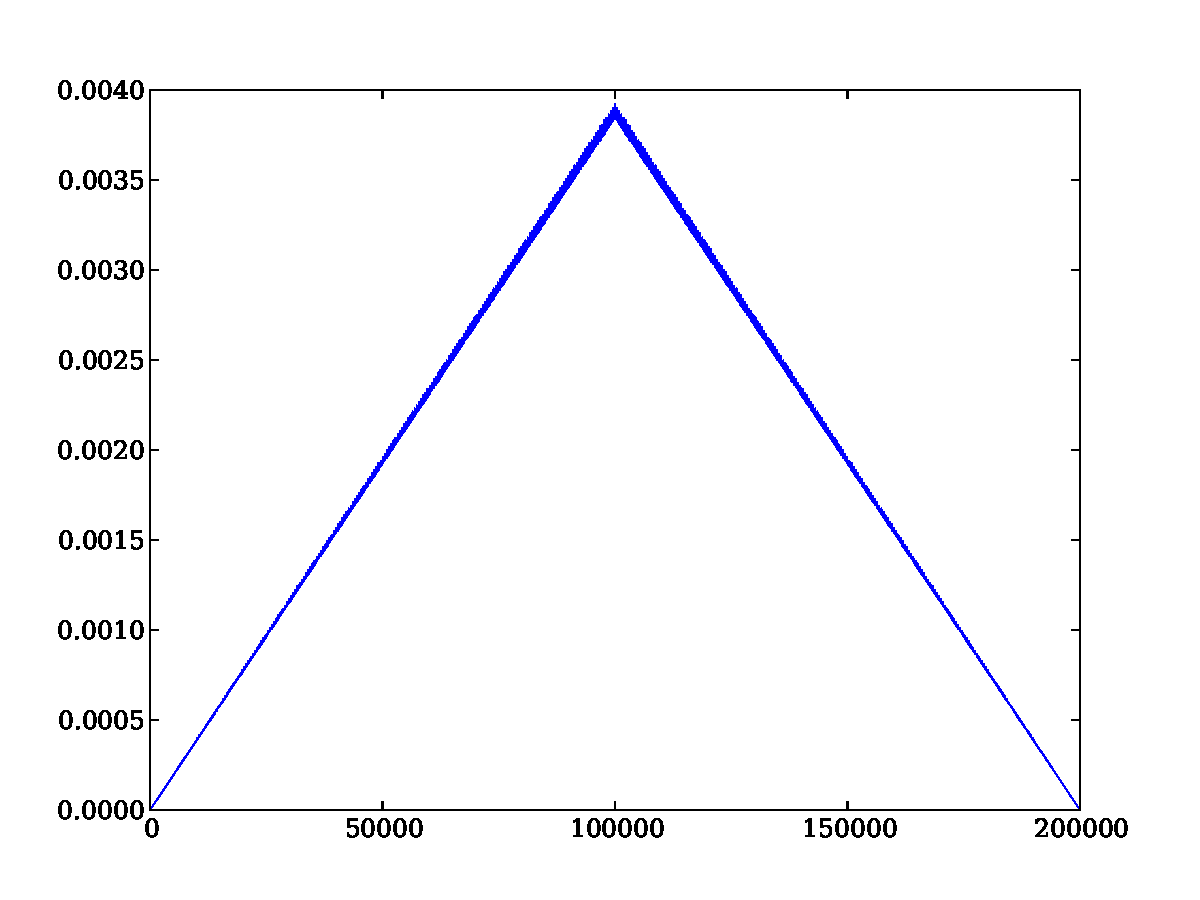
\includegraphics[width=\textwidth]{paulfigs/tcorr_J_1_266}
	\end{subfigure}
\end{figure}
\end{frame}

%-------------------------------------------------------------------------------

\begin{frame}
\frametitle{$g\tilde{J} = 1.2668$}
\begin{figure}
	\centering
	\begin{subfigure}[b]{0.49\textwidth}
		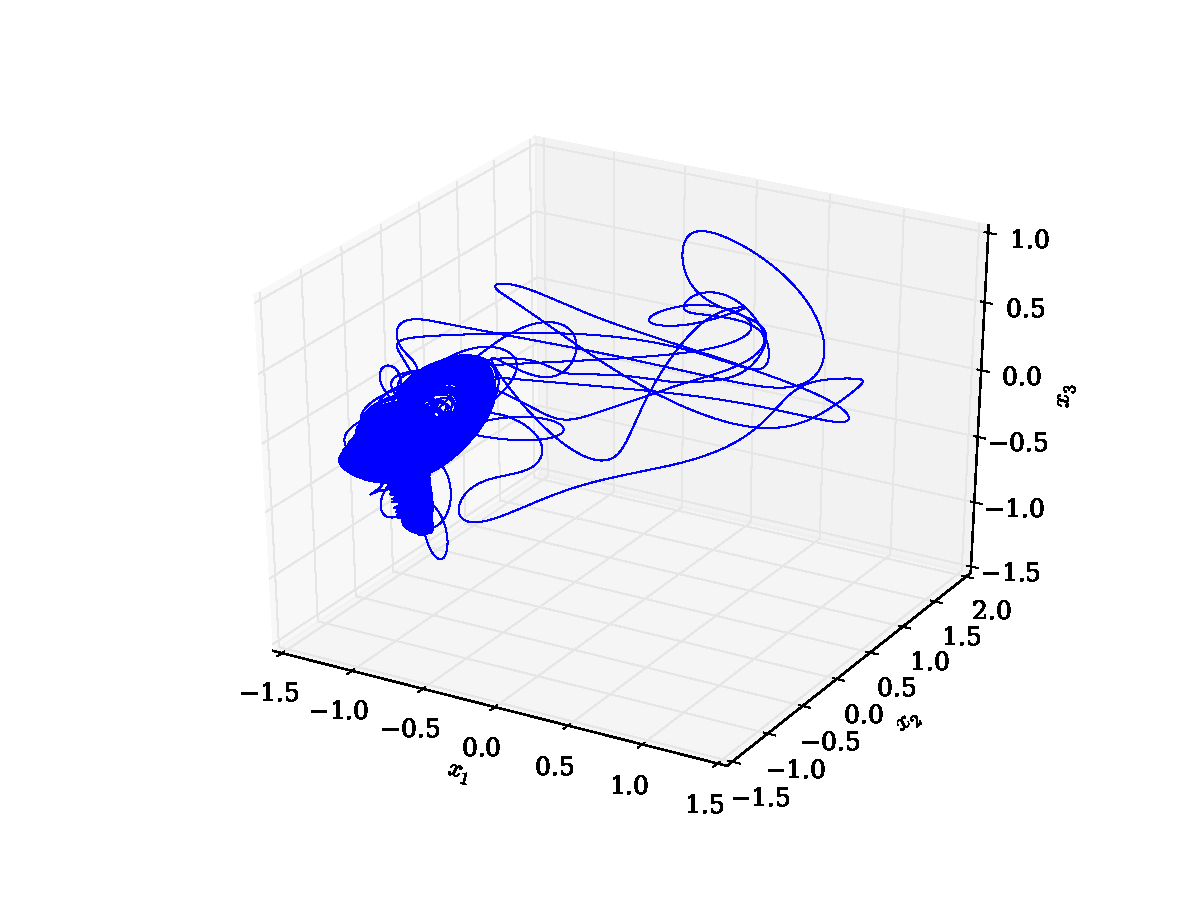
\includegraphics[width=\textwidth]{paulfigs/J_1_2668_3d}
	\end{subfigure}
	\begin{subfigure}[b]{0.49\textwidth}
		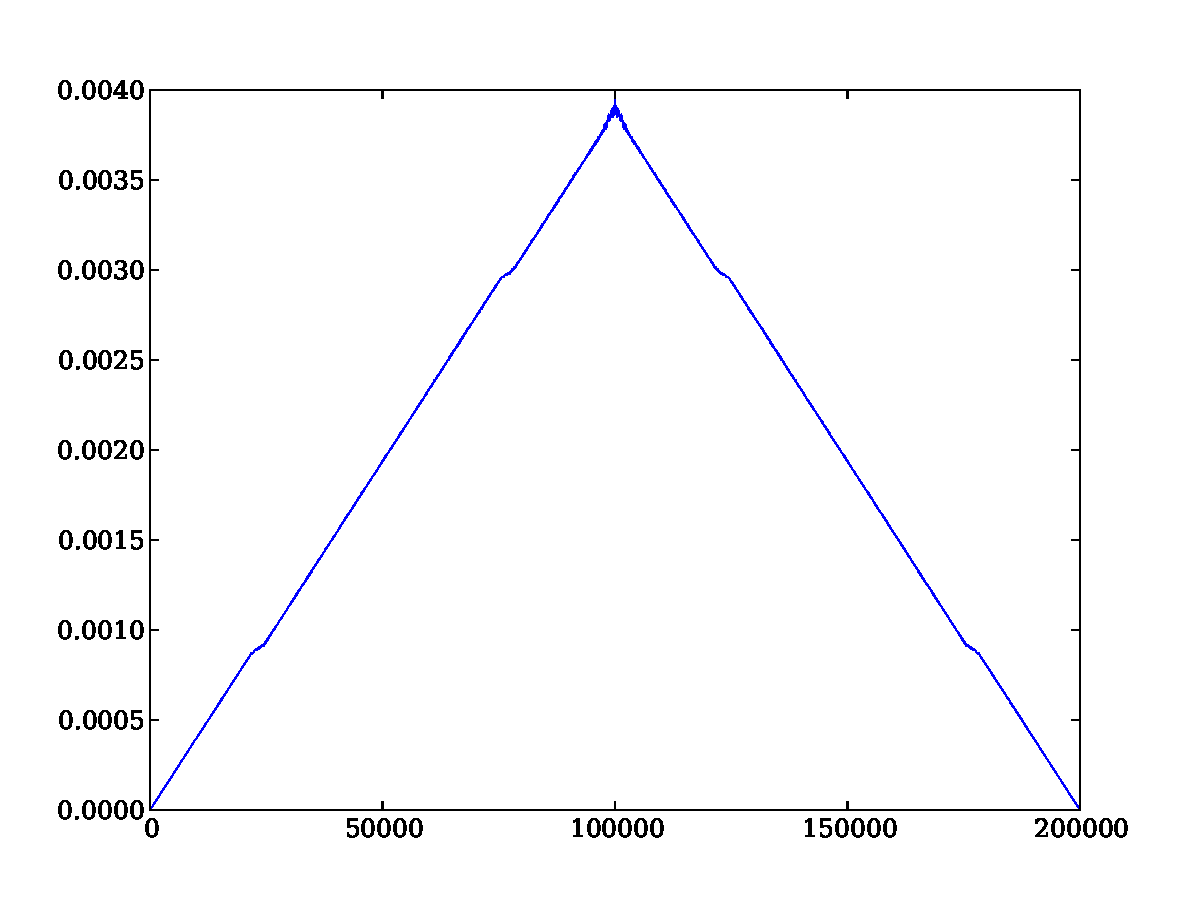
\includegraphics[width=\textwidth]{paulfigs/tcorr_J_1_2668}
	\end{subfigure}
\end{figure}
\end{frame}

%-------------------------------------------------------------------------------

\begin{frame}
\frametitle{$g\tilde{J} = 1.27$}
\begin{figure}
	\centering
	\begin{subfigure}[b]{0.49\textwidth}
		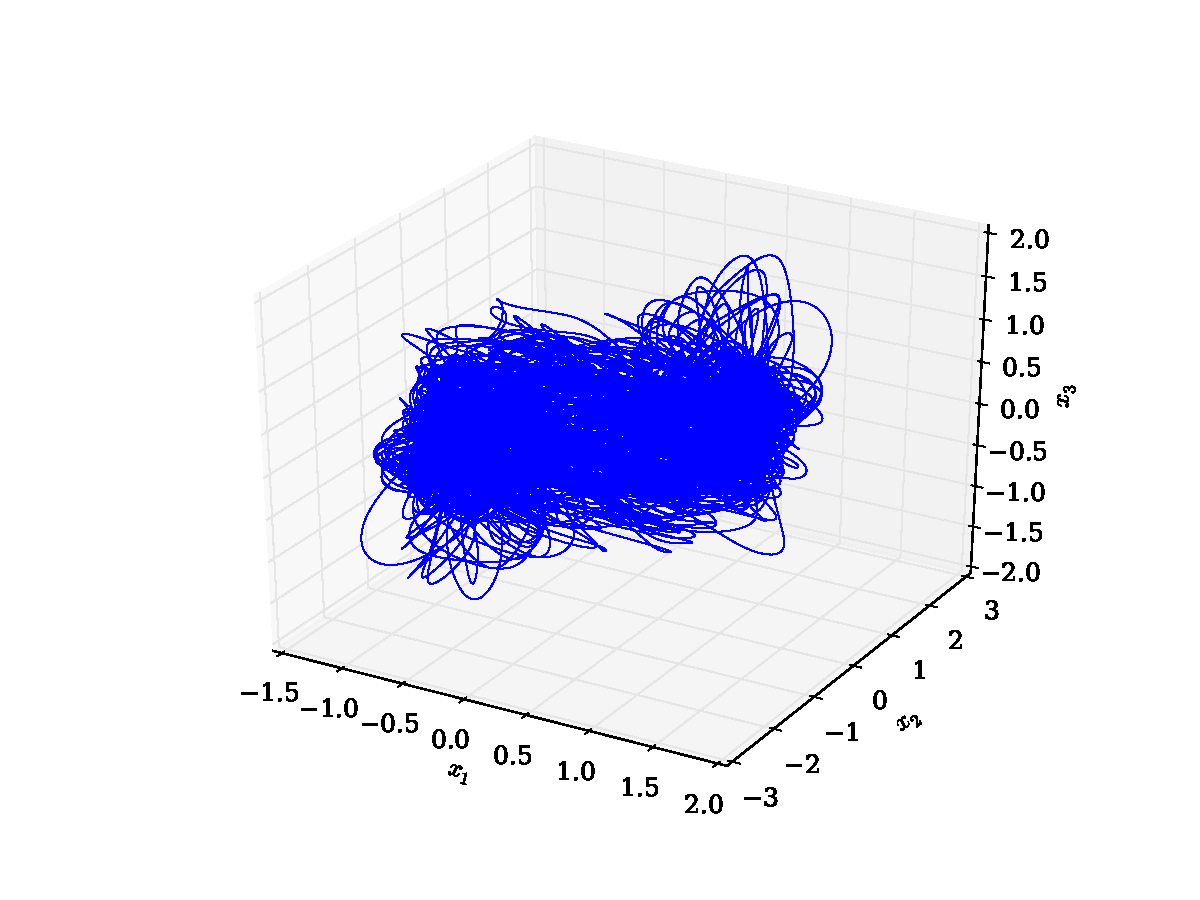
\includegraphics[width=\textwidth]{paulfigs/J_1_27_3d}
	\end{subfigure}
	\begin{subfigure}[b]{0.49\textwidth}
		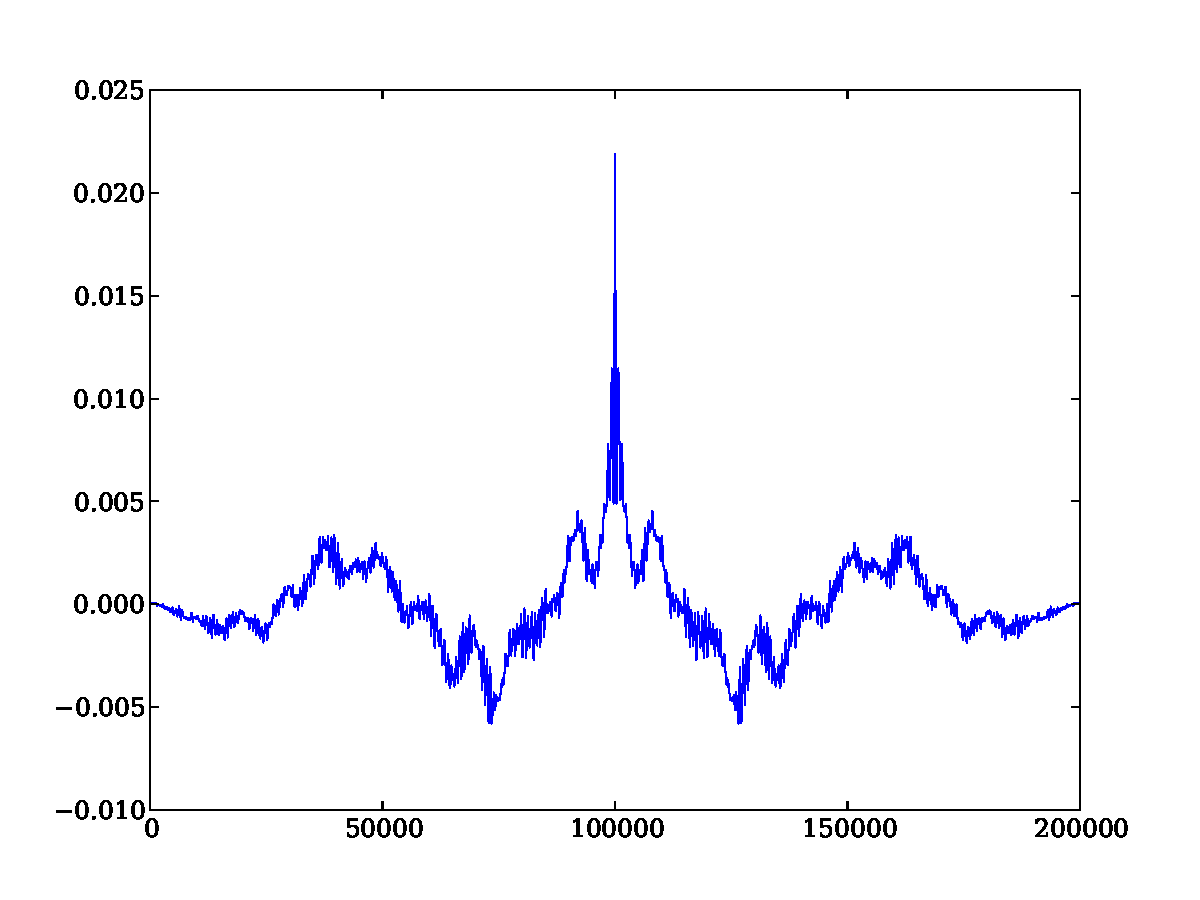
\includegraphics[width=\textwidth]{paulfigs/tcorr_J_1_27}
	\end{subfigure}
\end{figure}
\end{frame}

%-------------------------------------------------------------------------------

\begin{frame}
\frametitle{$g\tilde{J} = 1.3$}
\begin{figure}
	\centering
	\begin{subfigure}[b]{0.49\textwidth}
		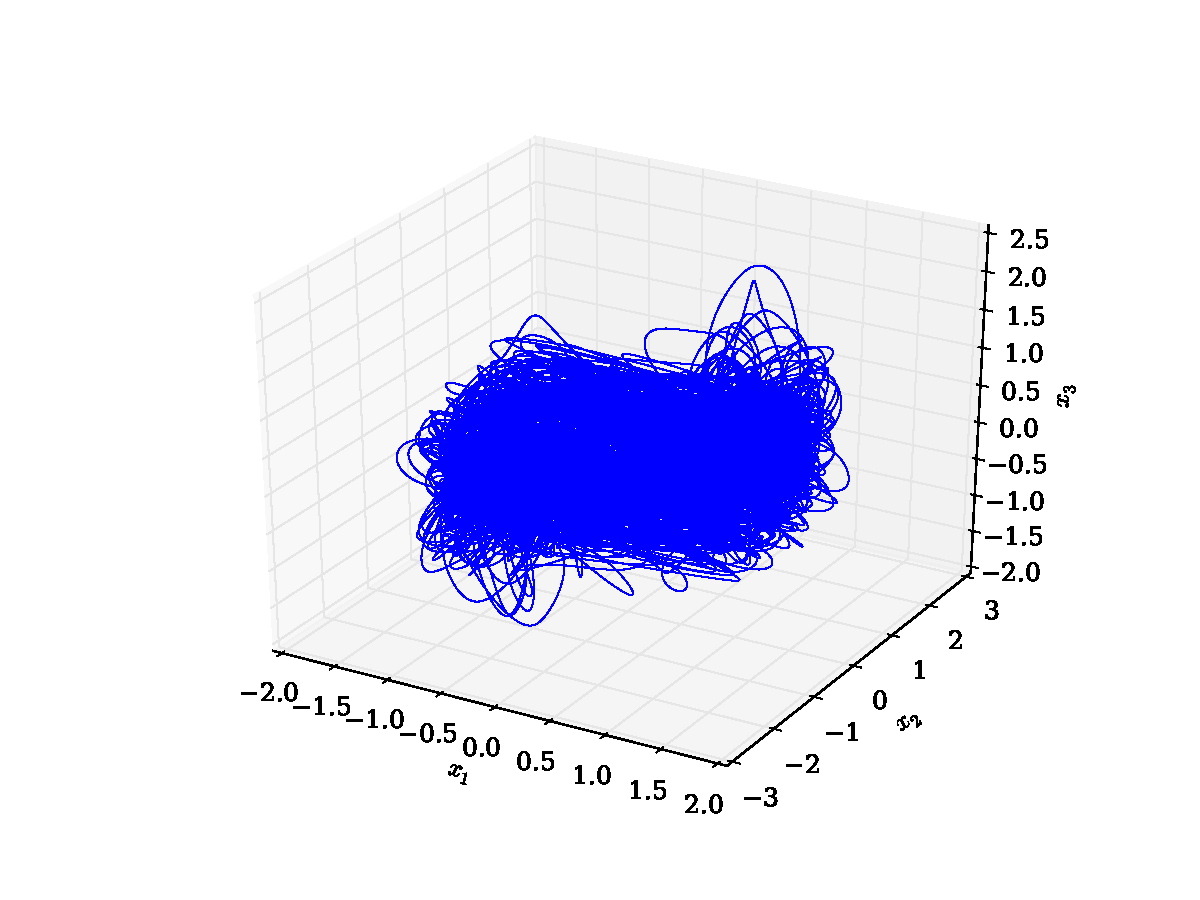
\includegraphics[width=\textwidth]{paulfigs/J_1_3_3d}
	\end{subfigure}
	\begin{subfigure}[b]{0.49\textwidth}
		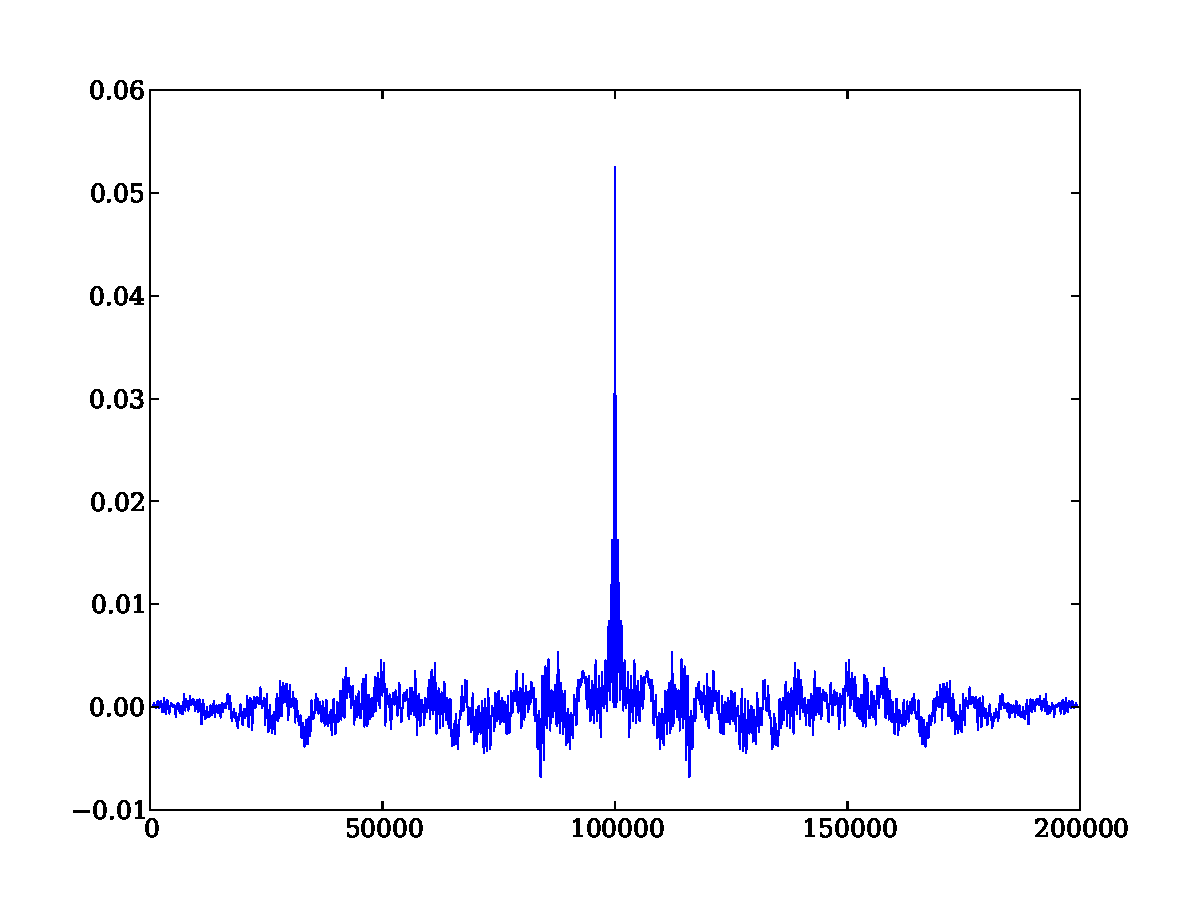
\includegraphics[width=\textwidth]{paulfigs/tcorr_J_1_3}
	\end{subfigure}
\end{figure}
\end{frame}


\end{document}









